In the second test, we prove the functionality of the algorithm in three dimensions. 

The algorithm compares the images and calculates the departure factor 
based on area of ROI. Fig. \ref{fig:target} demonstrates the 
tracking of $40$ images from initial position to the final position of the target, 
highlighted with red boxes;
the vector in blue describes the movement of the target. 

\begin{figure}[H]
\centering
  \subfloat[]{\label{fig:targeinit} \includegraphics[width=.48\columnwidth]{images/figurea.eps}}
  \subfloat[]{\label{fig:targeend} \includegraphics[width=.48\columnwidth]{images/figureb.eps}}
  \caption{The target in (a) is the initial position and its area is smaller than the target in (b), 
  which represents the final position. The factor is dividing both areas.}
  \label{fig:target}
\end{figure}

In Fig. \ref{fig:target}, we can observe an increase in ROI, and 
its influence to the departure factor is shown in Fig. \ref{fig:res_grapha_b}.

\begin{figure}[H]
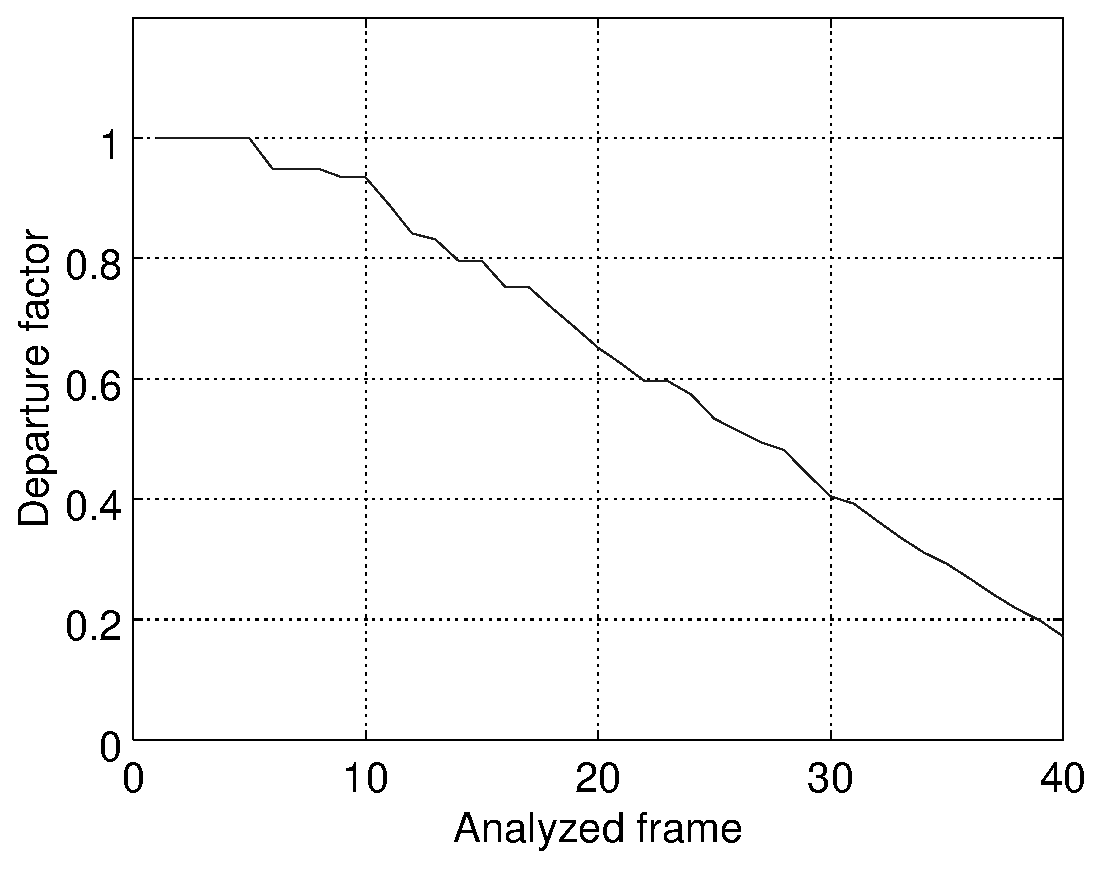
\includegraphics[width=\columnwidth]{images/grapha_b.eps}
\caption{Departure factor for each frame in the test 2.}
\label{fig:res_grapha_b}
\end{figure}

The Fig. \ref{fig:res_grapha_b} shows the departure factor in each frame
of test 2 (see the line with circles), additionally It is showed a polynomial
fitting of departure factor using a polynomial of order 4 (see the line with dots),
finally It is showed the real route of target normalized to $1.0$ for the maximum distance
(see the line with squares), as can be seen the target is approaching with a constant speed. 
If we interpret this value as the position in each sample time, 
then the departure factor describes the relative target position.
In the first image the analyzed target is at a distance $d_0$ 
and in the last image the target is at a distance of $17.18\%$ of $d_0$.
The departure distance decreases in discrete steps because the departure
factor is selected in discrete steps, if the target is
between two consecutive analysis layers (scales), the algorithm
approximates the target to the nearest layer.



The Table \ref{tab:tab1} represents the bank of images used for test 2, totally 40 images generated by POV-Ray.
The number of analyzed frames are in the first column of table, in the second column are the real distances 
between camera and target.
The percentage proportion of real distances are in third column. For example, 
the target in first frame is to $23.5$ meters from camera and it is considered the $100$\% of distance,
by other side, in the frame $40$ the target is to $4$ meters 
from camera and is $17,02$\% in relation of first frame. Next column, fourth column, 
we have the results of algorithm (departure factor), in the percentage form. 
%Note in first frame, target is $100$\% of distance and the last frame is at $17,18$\% of distance in relation of first frame.
Finally, the last column represents the error between percentage real distance and the departure factor. 
As can be seen, the error is diminishing when target is close (around 5 meters), it means that the algorithm has more precision 
when image of target is bigger because there are more information in ROI. It is a consequence of PCC, 
because in small ROI each pixel charge much information in comparative method. On other hand, if ROI is bigger,
the information is diluted around pixels; thus, the algorithm has more data to compare.
Another reason is that in the last frames $1$ pixel of target
represents a less distance in meters that $1$ pixel in the target of the first frames; consequently, the error 
of a quantity $x$ of pixels represents a less quantity of meters in the analysis of last frames.

\begin{table}[H]
\setlength{\tabcolsep}{1 pt} 
\caption{Table of comparative results}
\begin{tabular}{lllll}
Frames & Real Dist. (m) & Real Dist. (\%) & Dep. factor (\%) & Relative error (\%)\\
1 & 23.5 & 100.0 & 100.0 & 0.0 \\
10 & 19.0 & 80.85 & 93.46 & 15.60 \\
20 & 14.0 & 59.57 & 65.16 & 9.37 \\
30 & 9.0 & 38.30 & 40.46 & 5.65 \\
40 & 4.0 & 17.02 & 17.18 & 0.93
\end{tabular}
\label{tab:tab1}
\end{table}

The velocity of departure factor is shown in 
Fig. \ref{fig:res_grapha_bv}, where the velocity is calculated
to $d_0=1$ and $\Delta t=1$. The value of the departure
velocities is negative, which indicates that the
target is approaching towards the observer. Relative velocity is calculated 
using the discrete-time derivate.
If we compare test 1 and 2 to the same $\Delta t=1$, it is evident 
that the departure velocity of  test 2  is lower than test 1. 
Note target approaches more in test 2 and, consequently, departure
velocity is lower than test 1.
\begin{figure}[!hbt]
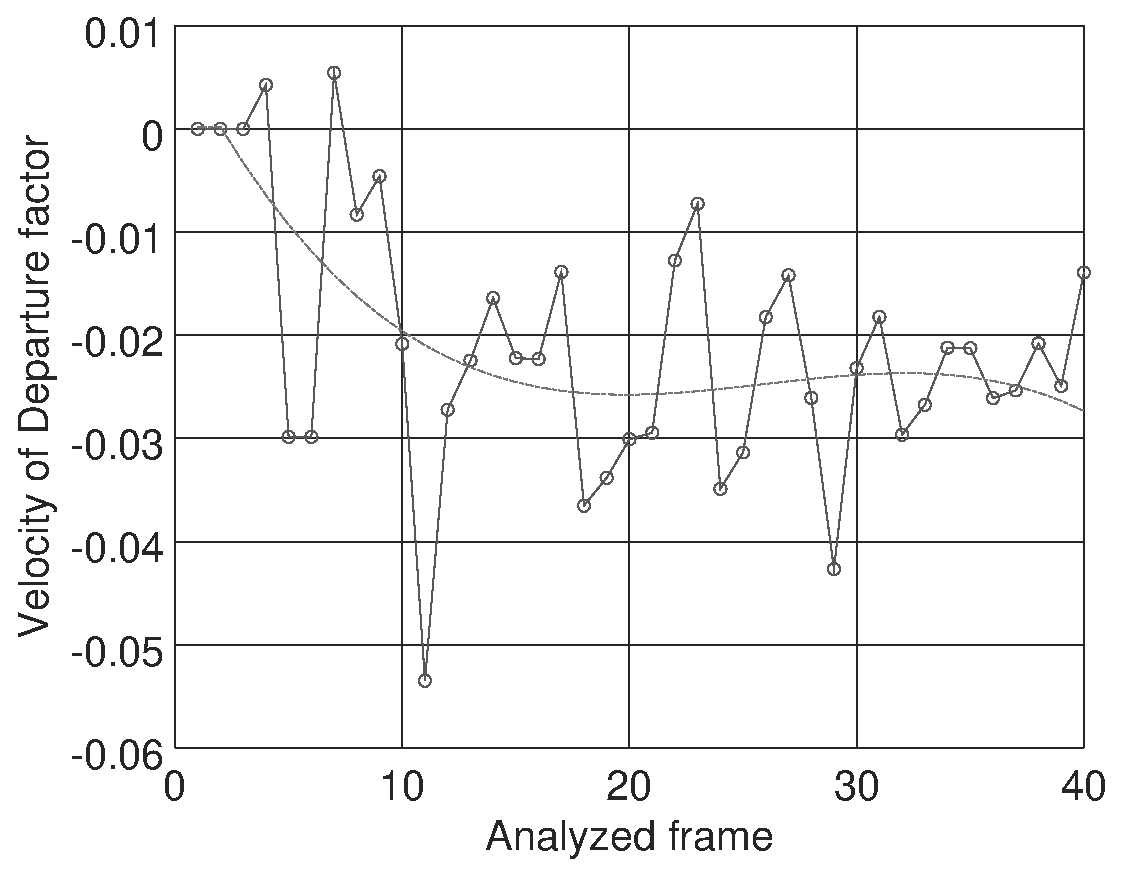
\includegraphics[width=\columnwidth]{images/graphvelocity.eps}
\caption{Velocity of departure factor for each frame in test 2.}
\label{fig:res_grapha_bv}
\end{figure}

